%% Preamble
  \documentclass{article}

  \usepackage[T1]{fontenc} % Use 8-bit encoding that has 256 glyphs
  \usepackage{fourier} % Use the Adobe Utopia font for the document - comment this line to return to the LaTeX default
  \usepackage[english]{babel} % English language/hyphenation
  \usepackage{amsmath,amsfonts,amsthm} % Math packages
  \usepackage{fancyhdr} % Required for custom headers
  \usepackage{lastpage} % Required to determine the last page for the footer
  \usepackage{extramarks} % Required for headers and footers
  \usepackage[pdftex]{graphicx}
  \usepackage{lipsum} % Used for inserting dummy 'Lorem ipsum' text into the template
  \usepackage{hyperref} % Used to add links to websites to the pdf
  \hypersetup{colorlinks,linkcolor=cyan,urlcolor=blue,citecolor=black}  % From Rick
  \usepackage{xifthen}
  \usepackage{booktabs}
  \usepackage{mdframed}

  % Margins
  \topmargin=-0.45in
  \evensidemargin=0in
  \oddsidemargin=0in
  \textwidth=6.5in
  \textheight=9.0in
  \headsep=0.25in

  \linespread{1.1} % Line spacing

  % Set up the header and footer
  \pagestyle{fancy}
  \lhead{\hmwkAuthorName} % Top left header
  \chead{\hmwkClass\ (\hmwkClassInstructor) \hmwkTitle} % Top center header
  \rhead{\firstxmark} % Top right header
  \lfoot{\lastxmark} % Bottom left footer
  \cfoot{} % Bottom center footer
  \rfoot{Page\ \thepage\ of\ \pageref{LastPage}} % Bottom right footer
  \renewcommand\headrulewidth{0.4pt} % Size of the header rule
  \renewcommand\footrulewidth{0.4pt} % Size of the footer rule
  \setlength\parindent{0pt} % Removes all indentation from paragraphs

  %%   DOCUMENT STRUCTURE COMMANDS
  % Header and footer for when a page split occurs within a problem environment
  \newcommand{\enterProblemHeader}[1]{
  \nobreak\extramarks{#1}{#1 continued on next page\ldots}\nobreak
  \nobreak\extramarks{#1 (continued)}{#1 continued on next page\ldots}\nobreak
  }

  % Header and footer for when a page split occurs between problem environments
  \newcommand{\exitProblemHeader}[1]{
  \nobreak\extramarks{#1 (continued)}{#1 continued on next page\ldots}\nobreak
  \nobreak\extramarks{#1}{}\nobreak
  }

  \setcounter{secnumdepth}{0} % Removes default section numbers
  \newcounter{homeworkProblemCounter} % Creates a counter to keep track of the number of problems

  \newcommand{\homeworkProblemName}{}
  \newenvironment{homeworkProblem}[1][Problem \arabic{homeworkProblemCounter}]{ % Makes a new environment called homeworkProblem which takes 1 argument (custom name) but the default is "Problem #"
  \stepcounter{homeworkProblemCounter} % Increase counter for number of problems
  \renewcommand{\homeworkProblemName}{#1} % Assign \homeworkProblemName the name of the problem
  \section{\homeworkProblemName} % Make a section in the document with the custom problem count
  \enterProblemHeader{\homeworkProblemName} % Header and footer within the environment
  }{
  \exitProblemHeader{\homeworkProblemName} % Header and footer after the environment
  }

  \newcommand{\problemAnswer}[1]{ % Defines the problem answer command with the content as the only argument
  \noindent \begin{mdframed} #1 \end{mdframed} % Makes the box around the problem answer and puts the content inside
  }

  \newcommand{\homeworkSectionName}{}
  \newenvironment{homeworkSection}[1]{ % New environment for sections within homework problems, takes 1 argument - the name of the section
  \renewcommand{\homeworkSectionName}{#1} % Assign \homeworkSectionName to the name of the section from the environment argument
  \subsection{\homeworkSectionName} % Make a subsection with the custom name of the subsection
  \enterProblemHeader{\homeworkProblemName\ [\homeworkSectionName]} % Header and footer within the environment
  }{
  \enterProblemHeader{\homeworkProblemName} % Header and footer after the environment
  }


  %   NAME AND CLASS SECTION
  \newcommand{\hmwkTitle}{Assignment\ \#1 - Math Review} % Assignment title
  \newcommand{\hmwkDueDate}{Friday,\ May\ 10,\ 2013} % Due date
  \newcommand{\hmwkClass}{Physics\ 441} % Course/class
  \newcommand{\hmwkClassInstructor}{Berrondo} % Teacher/lecturer
  \newcommand{\hmwkAuthorName}{Spencer Lyon} % Your name

  %   TITLE PAGE
  \title{
      \vspace{2in}
      \textmd{\textbf{\hmwkClass:\ \hmwkTitle}}\\
      \normalsize\vspace{0.1in}\small{Due\ on\ \hmwkDueDate}\\
      \vspace{0.1in}\large{\textit{\hmwkClassInstructor}}
      \vspace{3in}
  }

  \author{\textbf{\hmwkAuthorName}}
  \date{} % Insert date here if you want it to appear below your name

% New commands I use a lot
  \newcommand{\bs}[1]{\ensuremath{\boldsymbol{#1}}}
  \newcommand{\cross}[2]{\ensuremath{\boldsymbol{#1} \times \boldsymbol{#2}}}

  % partial derivative as a fraction
  \newcommand{\fracpd}[2]{
    \ensuremath{\frac{\partial #1}{\partial #2}}
  }

\begin{document}

Assignment:

\begin{itemize}
  \item 1.2
  \item 1.4
  \item 1.9
  \item 1.12
  \item 1.13
  \item 1.16
  \item 1.18
  \item 1.19
\end{itemize}

% Problem 1
  \begin{homeworkProblem}
      1.2: Is the cross product associative? $$ (\cross{A}{B}) \times \bs{C} \stackrel{?}{=} \bs{A} \times (\cross{B}{C})$$ If so prove it, if not provide a counter example
      \vspace{.2in}

      \problemAnswer{ % Answer
        Let $\bs{A} = \bs{i} = <1, 0, 0>$, $\bs{B} = \bs{i} = <1, 0, 0>$, $\bs{C} = \bs{k} = <0, 0, 1>$.

        In this case $$ (\cross{A}{B}) \times \bs{C} =  (<0, 0, 0>) \times <0, 0, 1> = <0, 0, 0>$$

        and $$ \bs{A} \times (\cross{B}{C}) = <1, 0, 0> \times (<0, -1, 0>) = <0, 0, -1>$$

        This two aren't equal to the cross product is non associative. \qed
      }
  \end{homeworkProblem}

% Problem 2
    \begin{homeworkProblem}
      1.4: Use the cross product to find the components of the unit vector $\hat{n}$ that is normal to the plane passing through the following points:  $<1, 0 0>, <0, 2, 0>, <0, 0, 3>$.
      \vspace{.2in}
      \problemAnswer{ % Answer
         We need to find two vectors parallel to the plane. We can use $<1, -2, 0>$ and $<0, 2, -3>$. Now that we have those vectors we can take the cross product between them and normalize the resultant vector. $$<1, -2, 0> \times <0, 2, -3> = <6, 3, 2>$$

       Now we normalize this vector to make it a unit vector: $$ \frac{<6, 3, 2>}{\text{norm}(<6, 3, 2>)} = \frac{<6, 3, 2>}{7} = <0.86,  0.43,  0.29>$$ \qed
      }
  \end{homeworkProblem}

% Problem 3
  \begin{homeworkProblem}
    1.9: Find the transformation matrix $R$ that describes rotation by $120^{\circ}$ about an axis from the origin through the point $(1, 1, 1)$. The rotation is clockwise as you look down the axis toward the origin.
    \vspace{.2in}
    \problemAnswer{ % Answer
      The general form for the rotation matrix of a vector about an axis of direction $u$ is given below:
      $$R = \begin{bmatrix} \cos \theta +u_x^2 \left(1-\cos \theta\right) & u_x u_y \left(1-\cos \theta\right) - u_z \sin \theta & u_x u_z \left(1-\cos \theta\right) + u_y \sin \theta \\ u_y u_x \left(1-\cos \theta\right) + u_z \sin \theta & \cos \theta + u_y^2\left(1-\cos \theta\right) & u_y u_z \left(1-\cos \theta\right) - u_x \sin \theta \\ u_z u_x \left(1-\cos \theta\right) - u_y \sin \theta & u_z u_y \left(1-\cos \theta\right) + u_x \sin \theta & \cos \theta + u_z^2\left(1-\cos \theta\right) \end{bmatrix}.$$

      In our case $\theta = 120^{\circ}$ and $u = <1, 1, 1>$. Plugging those things in we get the following matrix:

      $$ R = \begin{bmatrix}
      1.   &  0.63 &  2.37 \\
      2.37 &  1.   &  0.63 \\
      0.63 &  2.37 &  1.
      \end{bmatrix} $$ \qed
    }
  \end{homeworkProblem}

% Problem 4
  \begin{homeworkProblem}
    1.12: The height of a certain hill (in feet) is given by $$ h(x, y) = 10(2xy - 3x^2 - 4y^2 0 18x + 28y + 12)$$ where $y$ is the distance (in miles) north, $x$ is the distance east of South Hadley.

    \begin{enumerate}
      \item Where is the top of the hill located?
      \item How high is the hill?
      \item How steep is the slope (in feet per mile) at a point 1 mile north and one mile east of South Hadley? In what direction is the slope steepest, at that point?
    \end{enumerate}

    \vspace{.2in}
    \problemAnswer{ % Answer
      To answer these questions we need the gradient $$\nabla h(x,y) = 10\left((2y - 6x - 18) \hat{x} + (2x - 8y + 28) \hat{y}\right)$$
      \begin{enumerate}
        \item The top of the hill is where $\nabla h(x, y) = 0$. To find this we set each component equal to $0$ and solve the linear system.
        \begin{align*}
          0 &= 10\left((2y - 6x - 18) \hat{x}\right) \\
            & = 2y - 6x - 18 \\
            18 & = 2y - 6x
        \end{align*}

        \begin{align*}
          0 &= 10\left(  (2x - 8y + 28) \hat{y} \right) \\
            &= 2x - 8y + 28 \\
            -28 &= 2x - 8y
        \end{align*}

        We can now solve the equation $Ax=b$, where $A = \left(\begin{smallmatrix}  -6 & 2 \\ 2 & -8 \end{smallmatrix}\right)$,  $x = \left(\begin{smallmatrix} x \\ y \end{smallmatrix}\right)$, and $b = \left(\begin{smallmatrix} 18 \\ -28 \end{smallmatrix}\right)$

        This yields the solution that $x = -2, y = 3$, which means that the peak is 3 miles north and two miles west of South Hadley.

        \item For this part we just plug $(-2, 3)$ in to $h(x, y)$ and get $h^*(x, y) = h(-2, 3)  = 720$ ft.
        \item One mile north and one mile east of South Hadley means that $x = y = 1$. Plugging those into the gradient we get $$\nabla h(1, 1) = 10\left((2(1) - 6(1) - 18) \hat{x} + (2(1) - 8(1) + 28) \hat{y} \right) = 10 \left(-22 \hat{x} + 22 \hat{y} \right)$$

        The magnitude of this vector represents the steepness of the slope and is equal to $\sqrt{(-220)^2 + (220)^2} \approx 311.13$. Because the $x$ portion is negative and the $y$ portion is positive, the direction of steepest slope is northwest.
      \end{enumerate} \qed
    }
  \end{homeworkProblem}

% Problem 5
    \begin{homeworkProblem}
      1.13: Let $\bs{\eta}$ be the separation vector from a fixed point $(x', y', z')$ to hte point $(x, y, z)$ and let $\eta$ be its length. Show that:

      \begin{enumerate}
        \item $\nabla(\eta^2) = 2 \bs{\eta}$
        \item $\nabla(1 / \eta) = -\bs{\eta} / \eta^2$
        \item What is the general formula for $\nabla(\eta^n)$?
      \end{enumerate}

      \vspace{.2in}
      \problemAnswer{ % Answer
        We begin by defining $\bs{\eta}$ $$\bs{\eta} = (x - x') \hat{x} + (y - y') \hat{y} + (z - z') \hat{z} $$

        \begin{enumerate}
          \item We recognize that $\eta^2$ is simply the sum of each squared component: $$\eta^2 = (x - x')^2 + (y - y')^2 + (z - z')^2$$ We can now compute $\nabla(\eta^2)$

            \begin{align*}
              \nabla(\eta^2) &= \fracpd{\eta^2}{x} \hat{x} + \fracpd{\eta^2}{y} \hat{y} + \fracpd{\eta^2}{z} \hat{z} \\
                    &= 2(x - x')\hat{x} + 2(y - y')\hat{y} + 2(z - z')\hat{z}\\
                    &= 2 \bs{\eta}
            \end{align*}

          \item We know that $\eta = \sqrt{\eta^2} = \left((x - x')^2 + (y - y')^2 + (z - z')^2\right)^{1/2} $. Using this we can say that $(1 / \eta) =  \left((x - x')^2 + (y - y')^2 + (z - z')^2\right)^{-1/2}$. We will use this definition to solve the problem.
          Note that I define $\xi \equiv \left((x - x')^2 + (y - y')^2 + (z - z')^2\right)^{-3/2} \equiv \eta^{1/3}$. Also note that $\bs{\eta} = \eta \hat{\bs{\eta}}$

            \begin{align*}
              \nabla(1 / \eta) &= \fracpd{(1 / \eta)}{x} \hat{x} + \fracpd{(1 / \eta)}{y} \hat{y} + \fracpd{(1 / \eta)}{z} \hat{z} \\
                &= \frac{-1}{2} \xi 2(x - x') \hat{x} - \frac{1}{2} \xi 2(y - y') \hat{y}- \frac{1}{2} \xi 2(z - z') \hat{z}\\
                &= -\xi \left[(x - x') \hat{x} + (y - y') \hat{y} + (z - z') \hat{z} \right] \\
                &= - \eta^{1/3} \bs{\eta} = -\hat{\bs{\eta}} / \eta^2
            \end{align*}

          \item The general formula is pretty easy:

            \begin{align*}
              \nabla (\eta^n) &= n \eta ^{n-1} \fracpd{\eta}{x} + n \eta ^{n-1} \fracpd{\eta}{y} + n \eta ^{n-1} \fracpd{\eta}{z}\\
                &= n \eta ^{n-1} \left[ \frac{1}{2} \eta^-1 2 \eta_x + \frac{1}{2} \eta^-1 2 \eta_y + \frac{1}{2} \eta^-1 2 \eta_z\right] \\
                &= n \eta ^{n-1} \left[ \hat{\bs{\eta_x}} + \hat{\bs{\eta_y}}+ \hat{\bs{\eta_z}} \right] \\
                &= n \eta ^{n-1}  \hat{\bs{\eta}}
            \end{align*}

        \end{enumerate} \qed
      }
    \end{homeworkProblem}

% Problem 6
    \begin{homeworkProblem}
      1.16: Sketch the vector function $$\bs{v} = \frac{\bs{\hat{r}}}{r^2}$$ and compute its divergence. The ansewr may surprise you ... can you explain it?

      \begin{figure}[!h]
        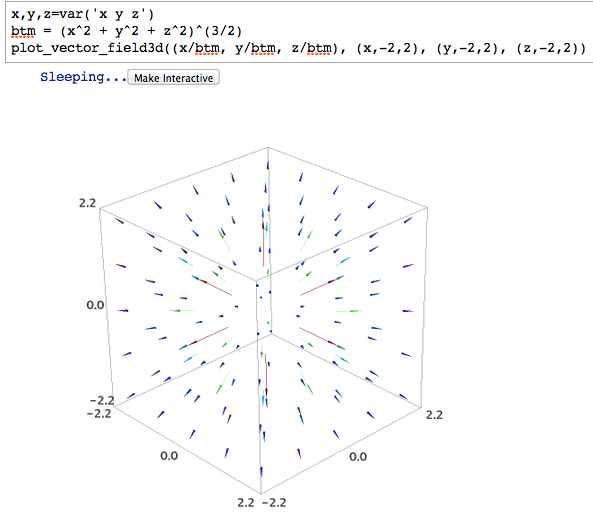
\includegraphics[width=\linewidth, height=4in]{VectorField.png}
        \caption{The vector field $\bs{v} = \frac{\bs{\hat{r}}}{r^2}$}
        \label{fig:b12Haz}
      \end{figure}

      \vspace{.2in}
      \problemAnswer{ % Answer

        For this problem $\bs{r} = x \hat{x} + y \hat{y} + z \hat{z}$ and  $r = \sqrt{x^2 + y^2 + z^2}$, so $\bs{v}$ becomes $$\bs{v} = \frac{\bs{\hat{r}}}{x^2 + y^2 + z^2} = \frac{\bs{r}}{(x^2 + y^2 + z^2) ^ {3/2}} = \frac{x \hat{x} + y \hat{y} + z \hat{z}}{(x^2 + y^2 + z^2) ^ {3/2}}$$

        The divergence can now be computed. Note that we make the substitution $\bs{\hat{r}} = \bs{r} / r$

        \begin{align*}
          \nabla \cdot \bs{v} &= \fracpd{\bs{v}}{x} + \fracpd{\bs{v}}{y} + \fracpd{\bs{v}}{z} \\
            &= \fracpd{(\bs{r} / r^3)}{x} + \fracpd{(\bs{r} / r^3)}{y} + \fracpd{(\bs{r} / r^3)}{z}\\
            &= \fracpd{}{x} \left[ x (x^2 + y^2 + z^2) ^{-3/2}\right] + \fracpd{}{y} \left[ y (x^2 + y^2 + z^2) ^{-3/2}\right] + \fracpd{}{z} \left[ z (x^2 + y^2 + z^2) ^{-3/2}\right] \\
            &=  3 (x^2 + y^2 + z^2) ^{-3/2} + (-3/2) (x^2 + y^2 + z^2) ^{-5/2} \left(2x^2 + 2y^2 + 2z^2 \right) \\
            &= 3 r^{-3}  - 3 r^{-5} \left( r^2\right)\\
            &= 3r^{-3} - 3r^{-3} = 0
        \end{align*}

        This is in the same form as Coulomb's law for a point charge. In this case the divergence represents the flux at a distance $r$. Because Coulomb's law describes point charges, the flux is zero for all radii not equal to 0. In other words, the only place flux exists is where the point charge is located. \qed
      }
    \end{homeworkProblem}

  \end{document}
